\begin{savequote}[75mm]
Some Quote.
\qauthor{Quoteauthor Lastname}
\end{savequote}

%For an example of a full page figure, see Fig.~\ref{fig:myFullPageFigure}.
\chapter{Model-Based Point Cloud Tracking}
\label{Chap:ModelBasedTracking}
\lettrine[lines=3, loversize=0.3]{\textcolor{DarkBlue}N}{ow that we have established} a reduced, stable world model in which voxels persist through occlusions, the next step is to adapt the general framework of Sequential Bayesian Estimation to track models within this 3D voxel model. The core concepts remain the same as discussed in Chapter \ref{Chap:VideoSegRelaxation}(for a brief introduction, see Appendix \ref{chap:SeqBayesEst}), and we will again use a bank of parallel particle filters, due to their robustness to noise (of which there is quite a bit in Kinect data) and ability to handle non-linear dynamics.

\section{Particle Filters in 3D}
The general concept of particle filtering remains the same as the 2D version discussed in Chapter \ref{Chap:VideoSegRelaxation}, with the primary changes lying in how we score individual particle predictions using the measurement model. The models have also been changed from 2D masks to 3D Point Cloud models which rely on point to point correspondence rather than a global histogram distance score. The dynamic model is an extension from 2D pixel position to real-world 3D coordinates which also include orientation. 

\section{Model Representation}
One of the main limitations of the 2D projected mask model discussed in Chapter \ref{Chap:VideoSegRelaxation} is that the masks of objects are not invariant to pose changes - in general, rotation of an object will change the shape of its mask and distribution of its color histogram. As we now have the ability to observe the full 3D shape of an object, we choose to represent objects as clusters of points which correspond to the exterior of the object. A visual representation of such a model is given in Figure \ref{fig:Object_Model}.

\missingfigure{Pointcloud representation of an object model}

Points for objects are stored in a model-centered reference frame (which we shall denote with superscript $^m$), with each point containing an XYZ position, an RGB color for the point, as well as a surface normal vector. That is, each point $p$ of the model $k$ consists of a nine-dimensional vector: 

\begin{equation} \label{eqn:point}
p^m_k = [x^m,y^m,z^m,R,G,B,n_x,n_y,n_z],
\end{equation}
 
 and a model for an object $O_k$ consists of a vector of $n_k$ such points $p^m$:
 
 \begin{equation} \label{eqn:model}
 O^m_k = [p^m_0 ... p^m_{n_k}].
\end{equation}

It is important to note that the points of an object model given above are model-relative - they must be transformed into the world coordinates in order to evaluate their fit to observations. This will be discussed further in the next Section.

\section{Dynamic Model}
\label{sec:Dynamic_model}
In the 2D tracker presented previously, the time-dependent state vector of a particle consisted of a position shift vector $\mathbf{p}_t=[p_x,p_y]$ and a velocity vector $\mathbf{v}_t=[v_x,v_y]$. The natural extension of this to 3D is to simply add a third $p_z$ and $v_z$ element to each. Of course we should note that the $x$ and$y$ dimensions here in our 3D representation are distinct from those in 2D, which represented pixel coordinates in the image plane. Here our positional coordinates represent real-world distances from a fixed origin (typically the camera ``pin-hole'' position). It is also important to note that coordinates in our 3D representation are originally in a continuous space - though we discretize them using the octree model discussed in the previous Chapter. For clarity, we shall simply denote coordinates in the world reference frame with no superscript.

While this straightforward extension gives us a reasonable 3D equivalent to our 2D tracked masks, we now have full 3D models, and so it makes sense to use a state vector which takes advantage of it. As such, we further extend the state vector for position and velocity to allow for rotations of the model around the object reference frame x-axis (roll - $\gamma$), y-axis (pitch - $\beta$), and z-axis (yaw - $\alpha$). This yields a position state vector for particle $j$ at time $t$ of 
\begin{equation} 
 \mathbf{x}^j_t = [d_x, d_y, d_z, \gamma, \beta, \alpha].
\end{equation}
Each object model is tracking using a set of $N$ such particles. We shall now generally omit the object variable $k$ in our notation for clarity. Even though we omit the $k$, the reader should assume that the following equations are for individual object models, and that we have a set of $N$ independent particles for each object.
Additionally, we have velocity state vector 
\begin{equation} 
 \mathbf{v}_t = [v_x, v_y, v_z, v_{\gamma}, v_{\beta}, v_{\alpha}],
\end{equation}
which is not tracked individually per particle, but rather as a whole for the model.

As before, motion is modeled using a constant velocity model in discrete time with a variable sampling period $\mathit{T}$, giving the dynamic model
\begin{equation} 
\mathbf{x}_t = \mathbf{x}_{t-1} + \mathit{T}\mathbf{v}_{t-1} + \mathbf{\omega} , 
\end{equation}
with noise vector $\mathbf{\omega}$ assumed to be zero mean Gaussian with fixed covariance.
Particle velocities are updated after weighting of individual particles using the measurement model, and are a weighted average of the change in position
\begin{equation} 
\label{Eqn:group_vel}
\mathbf{v}_t = \frac{1}{\mathit{T}N} \sum_{j=1}^{N} w_j (\mathbf{x}^j_{t} - \mathbf{x}^j_{t-1}), 
\end{equation}
where $w_j$ is the normalized weight for particle $j$. 

Tracking independent velocities for each particle doubles the dimensionality of the state-space, requiring a proportional increase in the number of particles. While the use of independent velocity states potentially helps in complicated tracking scenarios, in our experiments we were unable to observe any tangible benefit. Moreover, in order to avoid instability in the tracking results we needed to double the number of particles for a given noise level, doubling the processing time required. As such, we have chosen to use the above ``group-velocity'', and leave it to future work to investigate the possibility of independent velocity states.

\section{Measurement Model}
As points for the model are given in a model-centered frame of reference, we must transform them to the world frame them using a 3D affine transformation quaternion:
\begin{equation} \mathbf{B}^j = 
\begin{bmatrix}
 \cos{\alpha}\cos{\beta} & \cos{\alpha}\sin{\beta}\sin{\gamma} - \sin{\alpha}\cos{\gamma} & \cos{\alpha}\sin{\beta}\cos{\gamma} + \sin{\alpha}\sin{\gamma}  & d_x \\ 
\sin{\alpha}\cos{\beta} & \sin{\alpha}\sin{\beta}\sin{\gamma} + \cos{\alpha}\cos{\gamma} & \sin{\alpha}\sin{\beta}\cos{\gamma} - \cos{\alpha}\sin{\gamma}  & d_y \\ 
 -\sin{\beta} & \cos{\beta}\sin{\gamma} & \cos{\beta}\cos{\gamma} & d_z \\ 
 0 & 0 & 0 & 1
\end{bmatrix} \end{equation}
 which we use to transform the extended position vector for each point in the model:
\begin{equation} 
  p^m = [x^m,y^m,z^m,1],
\end{equation}
 yielding positions in the world frame for each of our $\eta$ model points for a particular particle $j$:
\begin{equation} 
  \begin{bmatrix}
    \mathbf{p}^j_1 \\
    \mathbf{p}^j_2 \\
    \vdots \\
    \mathbf{p}^j_\eta
  \end{bmatrix}
  \begin{bmatrix}
    [x_1,y_1,z_1,1]^\mathsf{T} \\
    [x_2,y_2,z_2,1]^\mathsf{T} \\
    \vdots    \\
    [x_\eta,y_\eta,z_\eta,1]^\mathsf{T}
  \end{bmatrix}
  =
  \begin{bmatrix} 
    \mathbf{B}^j & 0 & \ldots & 0 \\
    0 & \mathbf{B}^j & \ldots &  0 \\
    \vdots & \vdots & \ddots & \vdots \\
    0 & 0 & \ldots & \mathbf{B}^j 
  \end{bmatrix} 
  \begin{bmatrix}
    [x^m_1,y^m_1,z^m_1,1]^\mathsf{T} \\
    [x^m_2,y^m_2,z^m_2,1]^\mathsf{T} \\
    \vdots    \\
    [x^m_\eta,y^m_\eta,z^m_\eta,1]^\mathsf{T}
  \end{bmatrix}.
\end{equation}

Once we have our transformed points, we then must establish correspondences between each particle's model points and a world point. This is done so that we may score how well a particular particle matches the current world model observation. That is, for each transformed point $\mathbf{p}^j_{1\dotso \eta}$, we select corresponding point $\mathbf{p}^*$ in the observation which has minimal spatial distance.
\todo[inline]{Do I need to put an equation formalizing this? Maybe a figure?}
To find these correspondences, we first compute a KD-tree in the spatial dimensions for the world model points. This allows us to efficiently search for the nearest point to each transformed point. We create this tree for the world model rather than the transformed model (even though the former has more points) as there is only one world, but many particles and models. Computing it for the models would require a KD-tree for each particle in each model. Additionally, computing it for the world allows us to take advantage of sampling strategies (discussed later in this Chapter) which significantly reduce our run-time complexity. 

Once we have selected (with replacement) an observed point correspondence for each model point, we must calculate an un-normalized weight $\tilde{w}^j$ corresponding to the similarity of the transformed points to the world observation. This is accomplished   by summing the individual correspondence scores computed using weighted distance in world-, color-, and normal-space:
\begin{equation} \label{eqn:distance}
  \tilde{w}^j = \sum_{1}^{\eta} \frac{1}{1 + \frac {\mu \lVert \mathbf{p}^j_{xyz} - \mathbf{p}^*_{xyz} \rVert} {R_{voxel}} +  \frac{\lambda D_c(p^j_{RGB},p^*_{RGB})}{m} +   \epsilon \lVert \mathbf{p}^j_{n_x n_y n_z} - \mathbf{p}^*_{n_x n_y n_z} \rVert}, 
\end{equation}
where we follow the convention given Section\ref{subsec:Features}. That is, $\mu$, $\lambda$, and $\epsilon$ are weighting constants, $D_c$ is euclidean distance in CIELab space, and $m$ is a normalizing constant. We do not normalize normals, as they are already unit vectors. In our experiments we typically set the weighting factors to $\mu=1$, $\lambda=2$, $\epsilon=1$, as this balances the scoring between color and geometric shape, and found experimentally that it produced consistently good tracking results. The calculated particle weights $\tilde{w}^j$ are then normalized, and a final state estimate can be computed by taking the weighted average of all particles
\begin{equation} 
\mathbf{x}_t = \sum_{j=1}^{N} w_j \mathbf{x}^j_{t}, 
\end{equation}
and the group-velocity can be computed using Equation~\ref{Eqn:group_vel}.

\section{Stratified Correspondence Sampling}
\todo[inline]{Provide simple experiment showing quality of track (maybe on VR Data) vs number of samples and particles.}
\todo[inline]{Also show result with occlusion? With some pure random samples added in?}
\section{Results on Virtual-Reality Data}
\begin{figure*}[!ht]
  \centering
  \includegraphics[width=\linewidth]{figures/Tracking/CombinedNoNoise.pdf}
  \caption[Tracked Output vs Ground Truth Artificial Sequence]{Tracked Output vs Ground Truth Artificial Sequence. The top panel shows position in terms of XYZ displacement and the bottom shows rotation in terms of geodesic. The location is generally tracked quite well, while the rotation is noisy due to the rotational symmetry of the two tracked objects (a bolt-angular and shaft).}
  \label{fig:CombinedNoNoise}
\end{figure*}

\begin{figure*}[!ht]
  \centering
  \includegraphics[width=\linewidth]{figures/Tracking/Action_Segmentation.pdf}
  \caption[Segmentation of Actions]{Segmentation of Cranfield Sequence into Keyframes - Tracked objects are monitored for when interactions between them occur, yielding keyframes which correspond to semantically important frames. Results here are shown for an artificial sequence with depth and RGB noise added.}
  \label{fig:ActionSegmentation}
\end{figure*}

\section{Results on Real Data}
In this section we present results on 10 different recordings of humans assembling the Cranfield benchmark. Recordings here 

